\documentclass[brazilian, landscape]{standalone}

\usepackage{babel}
\usepackage[utf8]{inputenc}
\usepackage[T1]{fontenc}
\usepackage{lmodern}

\usepackage{tikz}
\usetikzlibrary{calc}

\definecolor{colorbg}{HTML}{DEDCF8}

\tikzset{down hexa chain/.pic={
        \foreach \i in {1,...,#1} {
            \path [draw, pic actions] (0, -{2*(\i-1)*sin(60)}) --
            ++(60:1) --
            ++(0:1) --
            ++(-60:1) --
            ++(240:1) --
            ++(180:1) --
            ++(120:1);
        }
    }
}
\tikzset{up hexa chain/.pic={
        \foreach \i in {1,...,#1} {
            \path [draw, pic actions] (0, {2*(\i-1)*sin(60)}) --
            ++(60:1) --
            ++(0:1) --
            ++(-60:1) --
            ++(240:1) --
            ++(180:1) --
            ++(120:1);
        }
    }
}

\begin{document}
    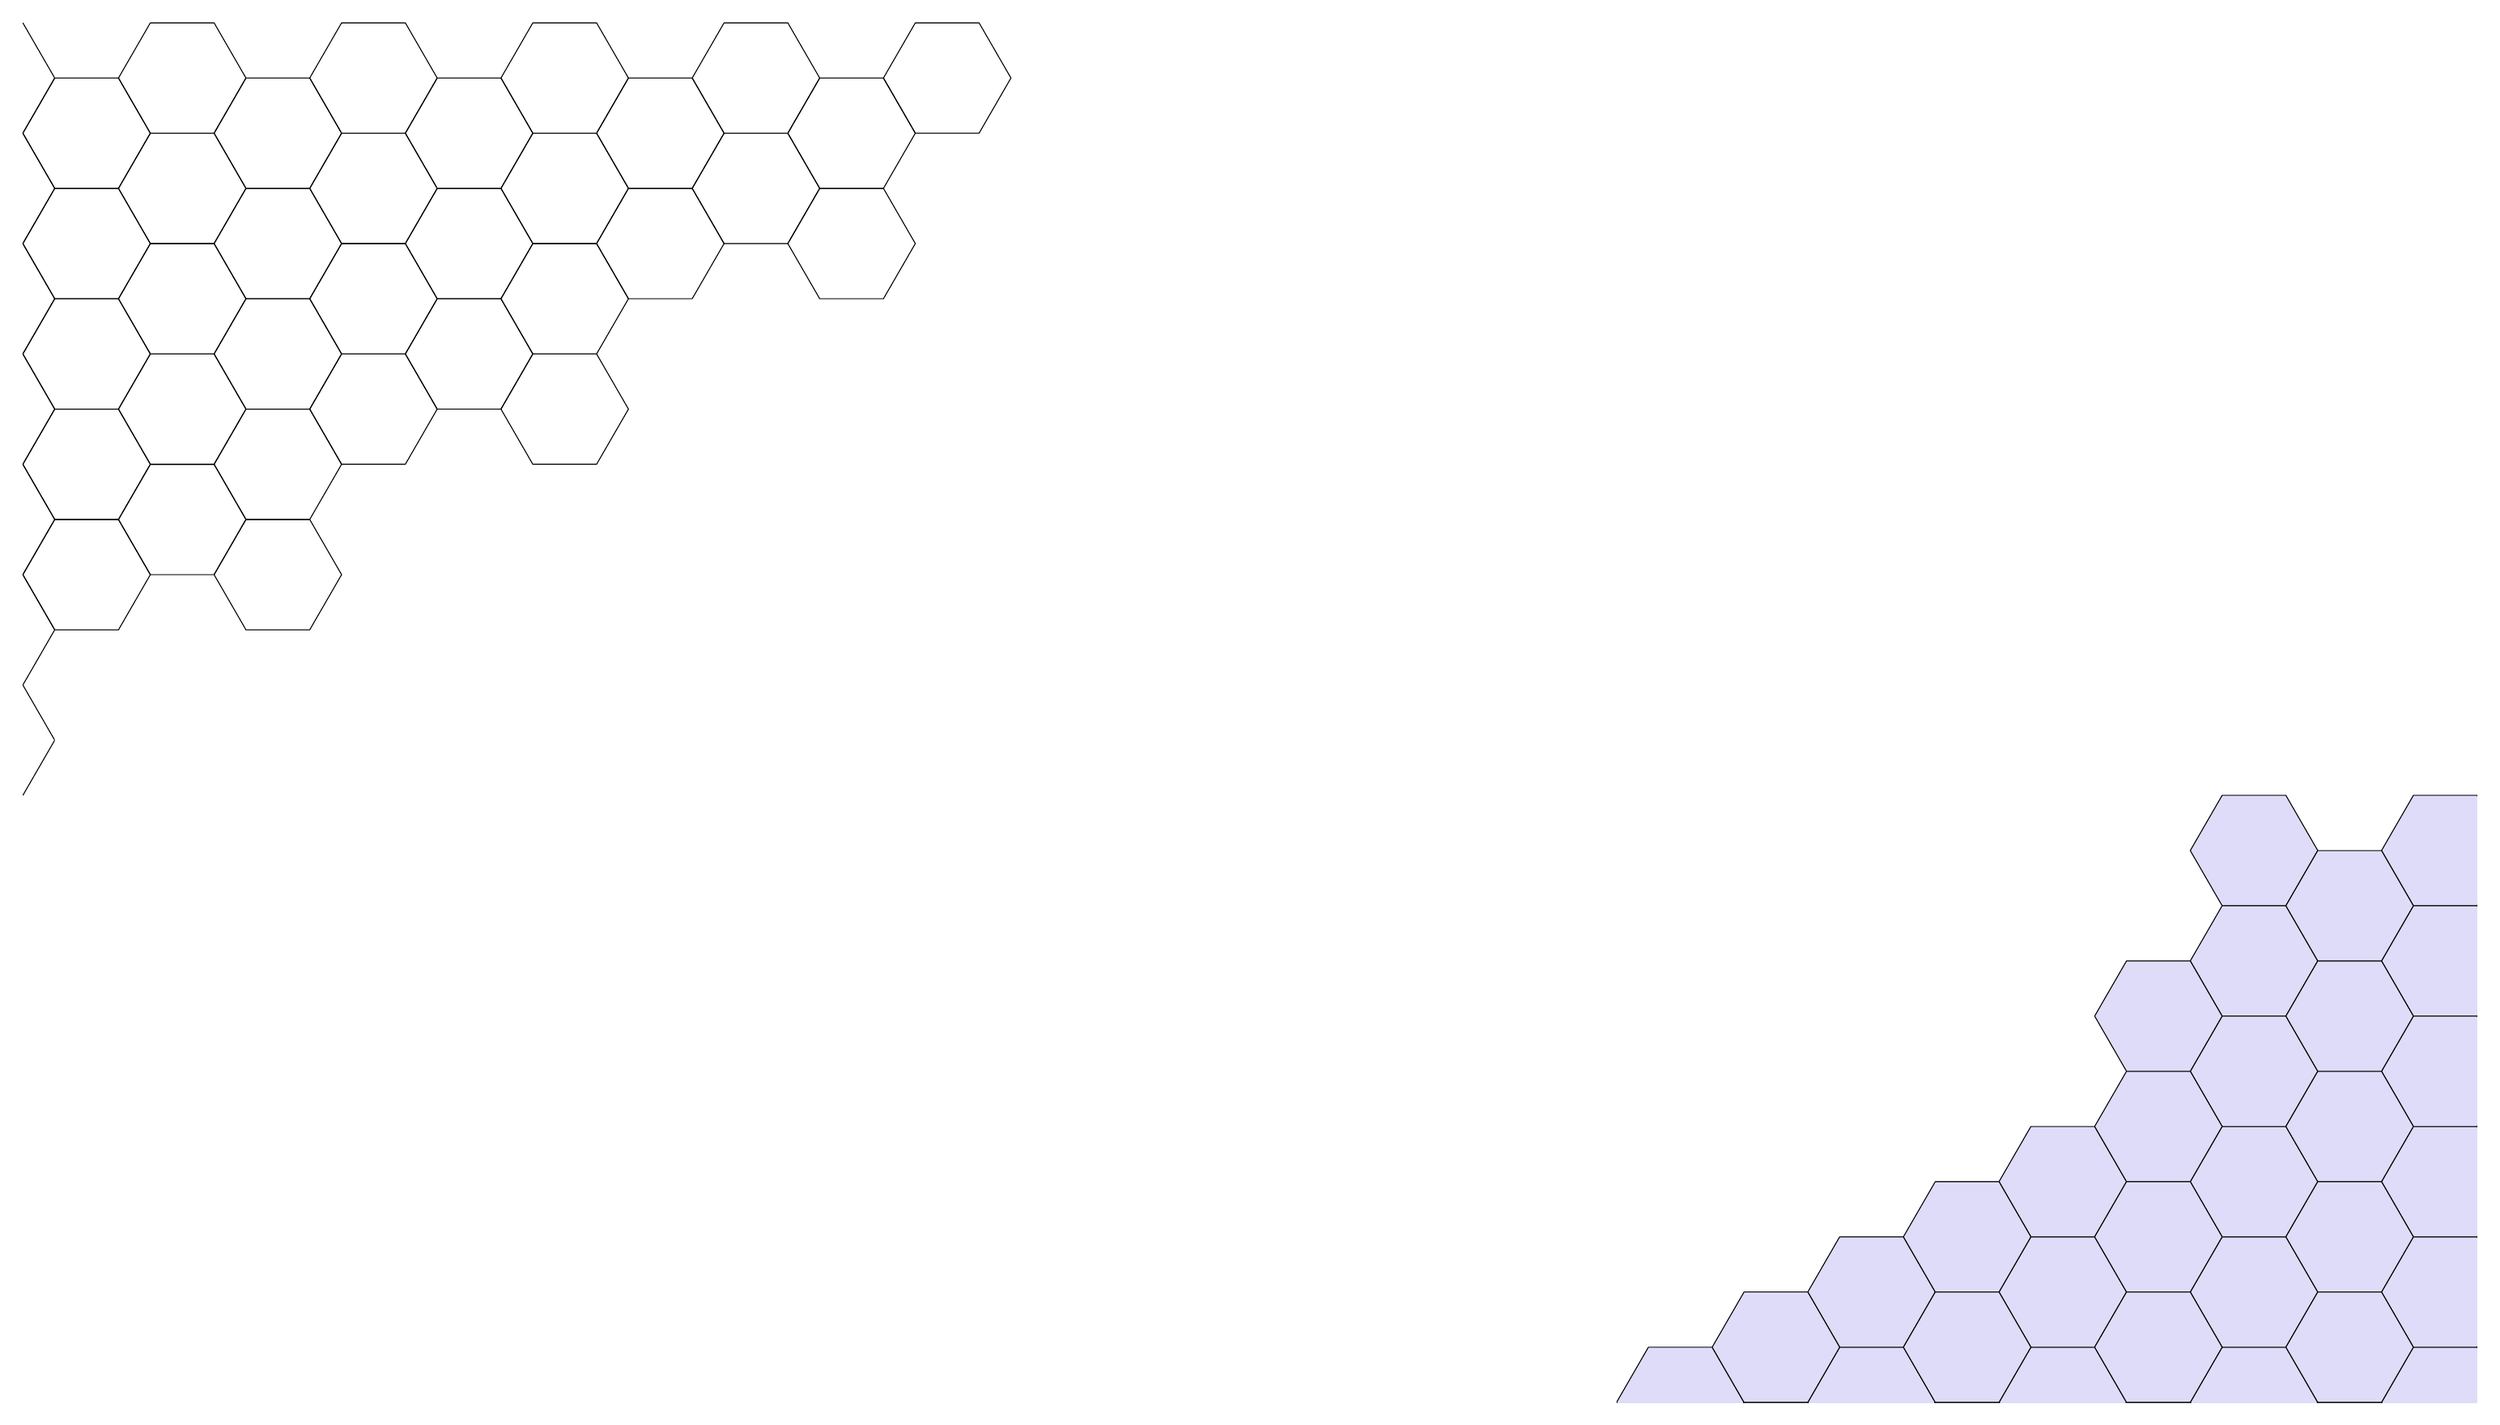
\begin{tikzpicture}
        \foreach \i/\j in {1/5,2/5,3/3,4/2,5/2} {
            \draw ({3*(\i-1)},0) pic {down hexa chain=\j};
        }

        \foreach \i/\j in {1/5,2/4,3/4,4/2,5/1} {
            \draw ({1.5+3*(\i-1)},{sin(60)}) pic{down hexa chain=\j};
        }

        \begin{scope}
            \clip (0,{2*sin(60)}) rectangle (0.5,{-12*sin(60)});

            \draw (-1.5,{sin(60)}) pic{down hexa chain=7};
        \end{scope}

        \begin{scope}[shift={(37,{-23*sin(60)})}, rotate=180]
            \clip (-1.5,0) rectangle ++(13.5,{-11*sin(60)-1});

            \foreach \i/\j in {1/6,2/6,3/3,4/2,5/1} {
                \draw ({3*(\i-1)},0) pic [fill=colorbg] {up hexa chain=\j};
            }

            \foreach \i/\j in {1/6,2/5,3/3,4/2} {
                \draw ({1.5+3*(\i-1)},{sin(60)}) pic [fill=colorbg] {up hexa chain=\j};
            }
        \end{scope}
    \end{tikzpicture}
\end{document}
